\chapter{绪论}[Introduction]

量子计算常被寄予厚望，但对于非本领域读者而言，一个更直接的问题往往是：它什么时候能在真实工程里产生可量化的收益？这个问题很难用一句话回答，因为量子计算的优势并不会以“通用加速器”的形式出现；更常见的情形是，它在某些结构特定的任务上，提供一种探索巨大状态空间或组合空间的新工具。\cite{Preskill2018NISQ}

近两年出现的一些工业试点与跨学科研究，为这种“结构特定的价值”提供了更直观的切入点。以移动通信网络为例，基站需要通过控制信令掌握终端位置并在来电时完成寻呼，这里面既包含大量统计数据，也包含带约束的组合优化：区域划分过细会导致终端频繁位置更新，过粗又会让寻呼覆盖范围过大，二者呈现典型的权衡关系。NTT~DOCOMO 在官方发布中报告，其基于量子退火平台开发的 ``TA-List 最适化'' 算法已在商用基站导入，并在特定区域实现了位置注册信号最高 $65.3\%$、寻呼信号最高 $7.0\%$ 的同时削减。\cite{Docomo2026TAListOptimization} 更早的联合试点则表明，在峰值时段寻呼信号可降低约 $15\%$，并给出了从 ``27~小时'' 级的通用求解到 ``40~秒'' 级混合求解的对比结果。\cite{NTTDocomoDWave2024QuantumOptimization,DWave2024DocomoCaseStory}

再以火灾防控为例，燃料隔离带（fuelbreak）的布局本质上是在复杂地形上选择少量干预线条，尽可能切断火势传播的连通性。Dent 等将地形抽象成网络图，并把 ``等分割'' 问题写成二次约束二进制优化（QCBO）形式，结合 D-Wave 的混合量子优化工具实现秒级求解，并在案例区域给出了相对传统 ``沿山脊布设'' 方法的改进方案。\cite{Dent2026WildfireFuelbreak} 这些结果并不等价于已经出现普适意义上的 ``量子优势''；但它们至少说明，量子算法与量子硬件正在从实验室 benchmark 走向更接近真实约束与真实数据的工程语境。\cite{Preskill2018NISQ,NationalAcademies2019QC}

应用愿景一旦落到工程层面，系统扩展压力就会变得具体而尖锐。当前多数平台仍处在 NISQ（Noisy Intermediate-Scale Quantum，噪声中等规模量子）阶段：可以演示一定规模的量子态制备与有限深度电路，但距离可纠错乃至容错量子处理器仍有明显差距。\cite{Preskill2018NISQ,NationalAcademies2019QC} 当目标从 ``做出更多物理比特'' 转向 ``持续运行的逻辑比特'' 时，制约因素往往不再是单个门的展示，而是控制与读出吞吐、稳定性、标定成本、误差传播，以及不同功能区之间的互连效率。\cite{NationalAcademies2019QC,Awschalom2021QuIC}

因此，模块化与分布式体系结构逐渐成为多平台共同关注的扩展路径。\cite{Jiang2007DistributedQC,Monroe2014ModularQC} 在这种架构里，本地模块承担高保真门操作与纠错，跨模块互连则通过光子信道建立可宣告的远程纠缠资源（通常是 Bell 对），再将其注入到更高层的纠错与计算流程。\cite{Monroe2014ModularQC,Covey2023QuantumNetworksNeutralAtomNodes} 承上启下的关键环节就是量子接口：它把驻留量子比特与飞行光子联系起来，并把发射、频率转换、传播、干涉、测量与前馈纳入统一的端到端误差链条。\cite{kimble2008quantum,NorthupBlatt2014QuantumInfoTransfer,Reiserer2022CavityEnhancedNetworkNodes}

本章旨在为后续建模工作建立清晰、易读的背景脉络。首先说明可扩展量子计算为什么会自然提出互连需求；随后解释量子接口的概念、主要实现路线与评价口径；再梳理典型平台的研究现状与优缺点；最后回到本文选取的 ``$^{87}$Rb--腔增强--频率转换--电信光纤--中继测量'' 链路，并说明端到端建模的必要性与全文结构安排。

\section{可扩展量子计算：为何需要互连}[Why scalable quantum computing needs interconnects]

\subsection{从应用案例到“规模化压力”}

从应用侧看，量子计算目前最成熟、也最常被讨论的方向之一是量子化学与多体量子模拟：量子系统本身的希尔伯特空间维数随粒子数指数增长，使得 ``用量子系统去模拟量子系统'' 在原理上更自然。\cite{Cao2019QuantumChemistry} 另一类更工程化的任务是组合优化与复杂网络决策：变量离散、约束繁多、可行解空间巨大，经典方法往往依赖启发式与大量工程经验。\cite{Preskill2018NISQ}

前述移动通信与火灾防控的例子，恰好属于后一类。为了降低理解门槛，这里用更直白的语言再概括一次其核心结构：第一类问题（通信网络）需要在 ``终端位置更新'' 与 ``来电寻呼覆盖'' 之间找到更好的折中，而折中的 ``划分方式'' 属于组合优化；第二类问题（燃料隔离带）需要在有限资源下选择 ``少量干预'' 来最大化 ``传播阻断''，同样可转写为组合优化。\cite{Docomo2026TAListOptimization,Dent2026WildfireFuelbreak} 这类问题通常并不要求量子态长期保持高深度电路，但要求求解器能在巨大组合空间里高效搜索，并能把约束自然地写进模型。\cite{Dent2026WildfireFuelbreak}

对量子计算硬件而言，真正困难的部分在于：一旦想把量子算法从 ``一次性演示'' 推进到 ``可复现、可迭代、可扩展''，系统就必须长期稳定地工作在更复杂的控制与读出闭环中。\cite{NationalAcademies2019QC} 这会引出一系列与读者直觉一致的工程矛盾：比特数越多，控制线和校准参数越多；并行度越高，时序同步与串扰管理越难；电路越长，误差累积越严重；而为了抑制误差又需要更频繁的测量与反馈，从而进一步挤压吞吐。\cite{Awschalom2021QuIC,NationalAcademies2019QC} 因而，可扩展量子计算在很大程度上是体系结构问题：它要求硬件、控制、互连与算法共同协同，而不是单个器件指标的简单堆叠。\cite{Wehner2018QuantumInternetVision}

\subsection{模块化与分布式量子计算简介}

模块化/分布式路线把 ``做更大的单机'' 变成 ``用更多可靠模块组成更大的系统''。\cite{Jiang2007DistributedQC,Monroe2014ModularQC} 在典型设想中，每个模块内部可以完成高保真本地门、测量与复位；模块之间通过光子链路建立远程 Bell 对，并用宣告信号（heralding）告诉我们 ``这一次连接成功了''，失败则丢弃并重试。\cite{Monroe2014ModularQC} 这种机制的优势在于：跨模块连接可以是概率性的，只要可宣告且可重复，就可以通过资源调度、复用和纠错把它转化为可用的计算资源。\cite{Jiang2007DistributedQC,Monroe2014ModularQC}

更广义的量子互联网愿景也强调了类似思路：未来的大规模量子信息系统更可能由功能不同、能力互补的节点组成，包括偏通信的节点、偏存储的节点与偏处理的节点。\cite{kimble2008quantum,Wehner2018QuantumInternetVision,Awschalom2021QuIC} 对本文关心的 ``处理中性原子节点'' 而言，本地里德伯门提供了可编程处理能力；跨模块互连则需要把少量通信比特与光场高效耦合，并通过中继站的双光子干涉与贝尔态测量（Bell-state measurement, BSM）建立远程纠缠。\cite{Covey2023QuantumNetworksNeutralAtomNodes,Sinclair2024FaultTolerantOpticalInterconnectsNeutralAtoms} 这里的 BSM 可理解为一种对 ``两光子联合态'' 的判别测量，它为远程纠缠提供 ``成功宣告''，同时把相位稳定需求从长距离光纤干涉转移到局域中继站。\cite{SimonIrvine2003RobustLongDistanceEntanglement}

\begin{figure}[htbp]
\centering
\begin{tikzpicture}[>=Latex,node distance=8mm and 10mm]
\tikzstyle{box}=[draw,rounded corners,align=center,minimum height=9mm,minimum width=28mm,font=\small]
\tikzstyle{widebox}=[draw,rounded corners,align=center,minimum height=9mm,minimum width=44mm,font=\small]
\node[box] (app1) {量子模拟\\量子化学};
\node[box,right=of app1] (app2) {优化\\采样/决策};
\node[box,right=of app2] (app3) {容错逻辑\\大规模算法};

\node[widebox,below=13mm of app2] (pressure) {规模、容错与吞吐需求上升};
\node[widebox,below left=13mm and 12mm of pressure] (mono) {单机扩展\\控制与互连压力};
\node[widebox,below right=13mm and 12mm of pressure] (mod) {模块化/分布式\\体系结构转向};

\node[box,below=15mm of mono] (memory) {存储节点};
\node[box,below=15mm of pressure] (comm) {通信节点};
\node[box,below=15mm of mod] (proc) {处理节点};

\node[widebox,below=15mm of comm] (interface) {量子接口：原子--光子映射、频率转换、传播、干涉、测量与前馈};

\draw[->,thick] (app1) -- (pressure);
\draw[->,thick] (app2) -- (pressure);
\draw[->,thick] (app3) -- (pressure);
\draw[->,thick] (pressure) -- (mono);
\draw[->,thick] (pressure) -- (mod);
\draw[->,thick] (mono) -- (memory);
\draw[->,thick] (pressure) -- (comm);
\draw[->,thick] (mod) -- (proc);
\draw[->,thick] (memory) -- (interface);
\draw[->,thick] (comm) -- (interface);
\draw[->,thick] (proc) -- (interface);
\end{tikzpicture}
\caption{可扩展量子计算中的 ``应用目标--体系结构转向--节点形态--量子接口需求'' 逻辑关系示意图。随着系统目标从小规模 NISQ 演示走向容错与大规模应用，单机扩展会逐渐遇到互连与吞吐瓶颈，进而推动模块化/分布式体系结构的发展；量子接口因此成为连接处理、存储与通信节点的关键耦合层。作者据相关文献整理绘制。\cite{Jiang2007DistributedQC,Monroe2014ModularQC,Wehner2018QuantumInternetVision,Awschalom2021QuIC,Covey2023QuantumNetworksNeutralAtomNodes}}
\label{fig:qc_architecture_logic}
\end{figure}

\section{量子接口：概念、任务与评价指标}[Quantum interfaces: concept, roles, and metrics]

\subsection{量子接口在网络化体系中的位置}

在本论文的语境中，量子接口更侧重指 ``处理节点--光信道--中继测量'' 这条链路中，负责量子态映射与条件化测量的一整层机制（它往往由多个器件共同构成，例如腔、频率转换器、滤波器和探测系统）。\cite{kimble2008quantum,NorthupBlatt2014QuantumInfoTransfer} 用更直观的表述来说：接口要把 ``驻留在原子/离子/固态自旋里的量子信息'' 可靠地装载到 ``可在光纤里飞行的光子'' 上，或反向把光子态写回到节点内部。\cite{Reiserer2022CavityEnhancedNetworkNodes,Awschalom2021QuIC}

从系统功能看，量子接口常见任务可以概括为三类。\cite{NorthupBlatt2014QuantumInfoTransfer,Awschalom2021QuIC} 第一类是纠缠产生：节点先制备物质--光子纠缠，再把来自不同节点的光子送到中继站干涉并做 BSM，从而把纠缠 ``交换'' 到远程物质比特上。\cite{Cabrillo1999CreationEntangledStates,SimonIrvine2003RobustLongDistanceEntanglement,vanleent2022entangling} 第二类是态转移与存储：把入射光子的量子态可逆写入物质体系，并在需要时读出，这为量子中继、同步等待与复用提供关键能力。\cite{Duan2001LongDistanceQuantumCommunication,Sangouard2011QuantumRepeatersAtomicEnsembles} 第三类是基于光的门操作或错误探测：利用散射/反射或腔增强相互作用，实现远程门、门传送或 error-detected 操作。\cite{Reiserer2022CavityEnhancedNetworkNodes,Grinkemeyer2025ErrorDetectedCavityNeutralAtoms}

\begin{figure}[htbp]
\centering
\begin{tikzpicture}[>=Latex,node distance=10mm and 10mm]
\tikzstyle{centerbox}=[draw,rounded corners,align=center,minimum height=10mm,minimum width=30mm,font=\normalsize]
\tikzstyle{branchbox}=[draw,rounded corners,align=left,minimum height=20mm,minimum width=42mm,font=\small,text width=42mm]
\node[centerbox] (core) {量子接口};

\node[branchbox,below left=18mm and 18mm of core] (ent) {纠缠产生\\
物质--光子纠缠 + 中继站干涉\\
产出：远程 Bell 对};
\node[branchbox,below=18mm of core] (mem) {态转移/存储\\
光 $\leftrightarrow$ 物质可逆映射\\
用途：缓存、同步、复用};
\node[branchbox,below right=18mm and 18mm of core] (gate) {门/错误探测\\
散射/腔相互作用/门传送\\
用途：远程门、容错资源};

\draw[->,thick] (core) -- (ent);
\draw[->,thick] (core) -- (mem);
\draw[->,thick] (core) -- (gate);
\end{tikzpicture}
\caption{量子接口在网络化体系中的三类典型任务示意图。三者并非互斥：同一平台往往会在不同体系结构阶段侧重不同任务。作者据相关文献整理绘制。\cite{NorthupBlatt2014QuantumInfoTransfer,Awschalom2021QuIC,Reiserer2022CavityEnhancedNetworkNodes}}
\label{fig:interface_tasks}
\end{figure}

\subsection{两类互连路线及评价口径}

远程纠缠产生型接口中，最常被对比的是 ``单光子'' 与 ``双光子干涉'' 两类方案。\cite{Cabrillo1999CreationEntangledStates,BarrettKok2005EfficientHighFidelityQC,SimonIrvine2003RobustLongDistanceEntanglement} 单光子方案可以在原则上把成功概率做得与单边链路效率线性相关，但通常对相位稳定提出更苛刻要求；双光子方案通过在中继站做两光子干涉与 BSM，把相位稳定需求局域化，更适合长光纤部署，但成功概率往往随两边链路效率呈二次缩放。\cite{SimonIrvine2003RobustLongDistanceEntanglement,vanleent2022entangling} 这里所谓 ``两光子干涉'' 常以 Hong--Ou--Mandel（HOM）干涉为直观代表：当两束不可区分单光子在分束器处相遇，会出现 ``同出同入'' 的量子干涉，其可见度直接反映波包在时间、频率、偏振与空间模式上的重叠程度。\cite{SimonIrvine2003RobustLongDistanceEntanglement}

\begin{figure}[htbp]
\centering
\begin{tikzpicture}[>=Latex,node distance=10mm and 10mm]
\tikzstyle{box}=[draw,rounded corners,align=center,minimum height=9mm,minimum width=32mm,font=\small]
\tikzstyle{smallbox}=[draw,rounded corners,align=center,minimum height=8mm,minimum width=26mm,font=\small]
\node[box] (nodeA) {节点 A\\(原子/离子)};
\node[box,right=30mm of nodeA] (nodeB) {节点 B\\(原子/离子)};
\node[smallbox,below=12mm of nodeA] (mid) {中继站};

\draw[->,thick] (nodeA) -- node[above,font=\small]{单光子方案：1 光子} (mid.west);
\draw[->,thick] (nodeB) -- node[above,font=\small]{单光子方案：本振/相位参考} (mid.east);

\node[smallbox,below=24mm of nodeA] (mid2) {中继站};
\draw[->,thick] (nodeA) -- node[above,font=\small]{双光子方案：A 光子} (mid2.west);
\draw[->,thick] (nodeB) -- node[above,font=\small]{双光子方案：B 光子} (mid2.east);
\draw[->,thick] (mid2) -- node[right,font=\small]{干涉 + BSM} ++(0,-8mm);
\end{tikzpicture}
\caption{单光子与双光子干涉型远程纠缠方案示意图。单光子方案对相位参考更敏感但成功率可线性受益于链路效率；双光子方案把相位稳定需求局域到中继站，更适合长光纤部署，但成功率对两边链路效率更敏感。作者据相关文献整理绘制。\cite{Cabrillo1999CreationEntangledStates,BarrettKok2005EfficientHighFidelityQC,SimonIrvine2003RobustLongDistanceEntanglement}}
\label{fig:single_vs_two_photon}
\end{figure}

在评价口径上，一个常见误区是只用 ``某个器件效率'' 来代表整条接口链路。更合理的系统级指标至少包括：尝试频率 $f_{\mathrm{rep}}$、单次尝试的宣告成功概率 $p_{\mathrm{succ}}$、单位时间纠缠建立率 $R_{\mathrm{ent}}=f_{\mathrm{rep}}p_{\mathrm{succ}}$，以及成功条件下的态保真度（或 CHSH 违背等量子相关见证量）。\cite{Reiserer2022CavityEnhancedNetworkNodes,Awschalom2021QuIC,Azuma2023QuantumRepeatersReview} 这些量并不会彼此独立：例如接受窗变宽可能提高 $p_{\mathrm{succ}}$，但也可能把更多背景计数纳入符合，从而拉低条件保真度；滤波变窄可以提升不可区分性与信噪比，却也可能带来额外损耗与时间记忆效应。\cite{Ikuta2018PolarizationInsensitiveQFC,vanleent2022entangling} 因而，端到端讨论通常需要同时给出 ``速率'' 与 ``质量''，并把噪声预算放在同一统计框架里。\cite{Zhou2023QuantumNetworkNoise}

\section{量子接口研究现状：主要平台与技术路线}[Research status: major platforms and routes]

\subsection{原子系综与量子存储：研究现状}

原子系综与量子存储路线是量子网络研究中最早形成系统技术树的一支。\cite{Duan2001LongDistanceQuantumCommunication,Sangouard2011QuantumRepeatersAtomicEnsembles} DLCZ 方案把原子系综、线性光学与单光子探测结合起来，为 ``先建立短程纠缠、再通过存储与交换延展距离'' 的量子中继思路奠定基础。\cite{Duan2001LongDistanceQuantumCommunication} 随后围绕存储效率、寿命、多模能力与读出保真度的研究逐渐成熟，形成 ``基于记忆的量子网络'' 路线。\cite{Sangouard2011QuantumRepeatersAtomicEnsembles,Zhu2025RemoteQuantumNetworksQuantumMemories}

在国内外研究进展中，原子系综路线长期占有重要位置。\cite{Sangouard2011QuantumRepeatersAtomicEnsembles,Zhu2025RemoteQuantumNetworksQuantumMemories} 国内在量子记忆与网络实验方面积累较深，既包括早期的远程原子系综量子记忆间隐形传态实验，也包括近年来面向真实城域链路的多节点量子网络验证。\cite{Bao2012TeleportationRemoteMemories,Liu2024MemoryMemoryEntanglementMetropolitanNetwork} 从读者角度理解，这些工作说明：``存储'' 不只是把光子延迟一会儿，它更像网络里的缓存与同步器，使概率性链路可以在更高层协议里被调度和复用。\cite{Azuma2023QuantumRepeatersReview}

这一路线的优势在于天然适合长距离网络中的等待与复用；其局限在于，若目标从 ``通信/存储'' 进一步转向 ``处理节点''，原子系综通常不如单离子或单原子寄存器那样便于实现高保真本地逻辑门与灵活的节点内计算。\cite{NorthupBlatt2014QuantumInfoTransfer,Covey2023QuantumNetworksNeutralAtomNodes} 因而，当前一个重要趋势并非相互替代，而是把存储型节点与处理型节点在体系结构层面重新分工。\cite{Wehner2018QuantumInternetVision,Awschalom2021QuIC}

\subsection{离子模块化节点：研究进展}

离子平台在高保真本地门、长相干时间与控制成熟度方面长期具有代表性，因此也是 ``处理节点 + 光子互连'' 思想最早被系统阐述的路线之一。\cite{Jiang2007DistributedQC,Monroe2014ModularQC} 分布式小寄存器理论与 MUSIQC 架构都强调：只要本地寄存器内部操作足够可靠，跨寄存器光学连接即使是概率性的，只要可宣告、可重复，就可以支撑大规模量子计算。\cite{Jiang2007DistributedQC,Monroe2014ModularQC}

实验上，离子体系通过 ``模块内声子总线 + 模块间光子总线'' 的层级结构较早展示了模块化互连可行性。\cite{Hucul2015ModularEntanglement} Hucul 等实现了借助光子和声子两种总线的模块化离子纠缠实验，说明局域确定性纠缠与远程概率性纠缠可以在同一平台内协同工作。\cite{Hucul2015ModularEntanglement} 读者可以把它理解为：模块内用 ``强、近、快'' 的相互作用做高保真门，模块间用 ``弱、远、可宣告'' 的光学链路做连接。\cite{Monroe2014ModularQC}

离子路线的长处在于体系结构叙事清楚且本地门质量高；其主要挑战在于远程光子接口的收集效率、系统复杂度以及大规模部署中的光学工程负担。\cite{Monroe2014ModularQC,NorthupBlatt2014QuantumInfoTransfer} 这些挑战并不削弱其作为 ``模块化处理节点'' 范式样板的价值，反而为中性原子、固态缺陷等平台提供了可借鉴的体系结构参照。\cite{Covey2023QuantumNetworksNeutralAtomNodes,Sinclair2024FaultTolerantOpticalInterconnectsNeutralAtoms}

\subsection{固态缺陷与量子点：进展与特点}

固态缺陷中心与量子点路线的吸引力主要来自集成潜力高、纳米光子兼容性好，以及更容易与电信基础设施对接。\cite{Awschalom2021QuIC} 在金刚石 NV/SiV 中心方向，Bernien 等较早实现了固态自旋量子比特之间的可宣告纠缠，Pompili 等进一步实现了三节点固态量子网络，在纠缠分发、纠缠交换与实时前馈方面迈出了关键一步。\cite{Bernien2013HeraldedEntanglement,Pompili2021MultinodeQuantumNetwork} 近期工作也展示了纳米光子金刚石腔与电信光纤网络的两节点量子网络，把多比特寄存器、腔增强与 telecom-compatible networking 更紧密地结合起来。\cite{Knaut2024NanophotonicNetwork,Bersin2024DiamondQuantumMemory}

量子点路线体现了另一类 ``发射体 + 频率转换 + 电信链路'' 的思路。\cite{DeGreve2012QuantumDotTelecom} De~Greve 等实现量子点自旋与光子的纠缠，并通过频率下转换把光子转到电信波段，展示了非原子体系也可与低损耗光纤窗口兼容。\cite{DeGreve2012QuantumDotTelecom} 同时也有工作探索电信光子与固态量子存储器的纠缠，为将来 ``电信光子直连存储'' 提供可能。\cite{Rakonjac2021TelecomPhotonSolidStateMemory}

这类平台在 ``高度集成'' 与 ``可制造'' 上很有吸引力，但其挑战也鲜明，包括谱线不均匀、材料涨落、频率漂移、低温需求与器件一致性等。\cite{Awschalom2021QuIC,Bersin2024DiamondQuantumMemory} 对读者而言，这可以理解为：固态路线更像 ``做芯片'' 的工程问题，而冷原子路线更像 ``做精密操控'' 的工程问题，两者难点不同。\cite{Covey2023QuantumNetworksNeutralAtomNodes}

\subsection{单原子与中性原子接口：腔增强与纳米光子路线}

单原子与中性原子路线近年升温的关键在于它开始同时吸收两类优势：一类来自冷原子与里德伯体系的长相干与可编程处理能力，另一类来自腔~QED 与纳米光子的高效率光子接口能力。\cite{Saffman2010QuantumInfoRydberg,KaufmanNi2021OpticalTweezerArraysNatPhys,Reiserer2022CavityEnhancedNetworkNodes} 早在单原子腔~QED 方向，Ritter 等就展示了 ``单原子嵌入光学腔'' 作为网络节点的基本图景：节点可以发送、接收、存储并再次释放量子光信息。\cite{Ritter2012ElementaryQuantumNetwork} Reiserer 的综述系统总结了腔增强节点如何提高原子--光子耦合强度、方向性与接口效率。\cite{Reiserer2022CavityEnhancedNetworkNodes}

与此同时，中性原子处理器本身也在快速成长。\cite{KaufmanNi2021OpticalTweezerArraysNatPhys} 光镊阵列带来单原子俘获与重排能力，里德伯相互作用提供强、可编程多体耦合，使中性原子平台在量子模拟与量子计算之间取得独特平衡。\cite{KaufmanNi2021OpticalTweezerArraysNatPhys} 近年代表性工作包括高保真并行纠缠门、基于可重构阵列的逻辑处理器，以及连续运行的千比特级相干系统，表明其正在从 ``可编程阵列'' 走向 ``处理器化节点''。\cite{Evered2023HighFidelityParallelRydbergGates,Bluvstein2024LogicalQuantumProcessor,Chiu2025ContinuousOperation3000Qubits}

当这一路线与量子网络问题汇合时，核心突破在于：把原子--光子纠缠真正推到电信光纤可用的距离尺度。\cite{Covey2023QuantumNetworksNeutralAtomNodes} van~Leent 等实现了原子--光子纠缠的电信波段分发，并在总长 $33\,\mathrm{km}$ 的电信光纤上实现单原子之间的纠缠建立；进一步的长寿命量子记忆把相关距离推到 $101\,\mathrm{km}$ 量级。\cite{vanleent2020longdistance,vanleent2022entangling,zhou2024longlived} 同期还有工作把光镊阵列与光学腔结合以实现可多路复用的网络寄存器，或推进原子阵列与纳米光子芯片集成。\cite{Hartung2024QuantumNetworkRegisterTweezerCavity,Menon2024IntegratedAtomArrayNanophotonicChip} 这些进展共同说明，中性原子网络接口已不再是单点演示，而是多条技术树在近几年开始交汇的结果。\cite{Sinclair2024FaultTolerantOpticalInterconnectsNeutralAtoms}

\begin{figure}[htbp]
\centering
\begin{tikzpicture}[>=Latex,node distance=8mm and 12mm]
\tikzstyle{root}=[draw,rounded corners,align=center,minimum width=28mm,minimum height=9mm,font=\small]
\tikzstyle{leaf}=[draw,rounded corners,align=left,text width=34mm,minimum height=15mm,font=\small]
\node[root] (root) {量子接口平台};

\node[leaf,below left=16mm and 18mm of root] (ensemble) {原子系综/量子存储\\
优点：缓存、多模、量子中继\\
挑战：处理能力有限};
\node[leaf,below left=38mm and 3mm of root] (ion) {离子/小寄存器\\
优点：本地门质量高、模块化清晰\\
挑战：远程光子接口速率};
\node[leaf,below right=38mm and 3mm of root] (solid) {固态缺陷/量子点\\
优点：纳米光子与芯片集成\\
挑战：材料同质性与漂移};
\node[leaf,below right=16mm and 18mm of root] (neutral) {单原子/中性原子\\
优点：本地处理 + 光接口并存\\
挑战：高效耦合与系统集成};

\draw[->,thick] (root) -- (ensemble);
\draw[->,thick] (root) -- (ion);
\draw[->,thick] (root) -- (solid);
\draw[->,thick] (root) -- (neutral);
\end{tikzpicture}
\caption{典型量子接口平台的技术树与优缺点概览。作者据相关文献整理绘制。\cite{Duan2001LongDistanceQuantumCommunication,Sangouard2011QuantumRepeatersAtomicEnsembles,Monroe2014ModularQC,Hucul2015ModularEntanglement,Bernien2013HeraldedEntanglement,Pompili2021MultinodeQuantumNetwork,Covey2023QuantumNetworksNeutralAtomNodes}}
\label{fig:platform_tree}
\end{figure}

\begin{table}[htbp]
\centering
\small
\renewcommand{\arraystretch}{1.25}
\caption{典型量子接口平台的系统级比较}
\label{tab:platform_compare}
\begin{tabular}{|p{2.2cm}|p{2.7cm}|p{4.3cm}|p{4.3cm}|}
\hline
平台类型 & 典型节点能力 & 主要优势 & 主要挑战 \\
\hline
原子系综/量子存储 & 光--物质量子态映射、缓存、中继 & 适合长距离网络、同步等待、多模与复用潜力较强 & 本地处理能力相对有限，难以直接承担复杂处理节点角色 \\
\hline
离子/小寄存器 & 高保真本地门、模块化互连 & 体系结构清晰，适合 ``本地确定性 + 远程宣告型'' 计算范式 & 光子收集与远程接口速率受限，系统复杂度较高 \\
\hline
固态缺陷/量子点 & 芯片级发射体、纳米光子耦合 & 易集成、可对接 telecom 与片上器件 & 谱线漂移、材料离散性、低温与制备一致性要求高 \\
\hline
单原子/中性原子 & 光镊阵列、本地门、腔/波导接口 & 本地处理能力与网络接口潜力可在同一平台上结合 & 需要同时解决高效收集、频率转换、链路噪声与系统集成 \\
\hline
\end{tabular}
\end{table}

\section{处理中性原子节点：本文选取的接口链路}[Neutral-atom processing nodes and the chosen link]

\subsection{处理中性原子节点的概念与需求}

本文所说的 ``处理中性原子节点''，指的是节点内部既拥有可编程多比特原子寄存器，也拥有能与光场高效耦合的通信自由度。\cite{Covey2023QuantumNetworksNeutralAtomNodes} 换成更工程化的语言：节点里一部分原子（或一部分受控模式）负责 ``通信''，用于产生原子--光子纠缠、接收光子、或把本地量子态映射到飞行光子；另一部分原子负责 ``计算''，用于本地门操作、错误检测/纠错与资源管理。\cite{Sinclair2024FaultTolerantOpticalInterconnectsNeutralAtoms}

这个定义强调了一个读者容易忽略的点：远程光学链路建立的是跨模块 Bell 对，而把 Bell 对变成分布式计算资源，需要节点内部的本地处理能力配合（例如做门传送、纠错注入或纠缠净化）。\cite{Monroe2014ModularQC,Covey2023QuantumNetworksNeutralAtomNodes} 因而，即使本文后续链路层面只模拟 ``两端各一个原子'' 的远程纠缠产生过程，它所对应的问题仍属于 ``处理节点如何接入网络'' 的接口层评估，而不是纯通信意义上的链路演示。\cite{Sinclair2024FaultTolerantOpticalInterconnectsNeutralAtoms}

\subsection{选取 \texorpdfstring{$^{87}$Rb--cavity--QFC--telecom--BSM}{87Rb--cavity--QFC--telecom--BSM} 链路的理由}

在众多可能实现中，$^{87}$Rb + 高精细度光学腔 + 量子频率转换（quantum frequency conversion, QFC）+ 电信光纤 + 中继站 BSM 这一路线具备较强的 ``代表性'' 与 ``可对照性''。\cite{vanleent2020longdistance,vanleent2022entangling,Reiserer2022CavityEnhancedNetworkNodes} 其中，$^{87}$Rb 是原子物理中最成熟的体系之一，能级结构、冷却俘获与选择规则清楚，实验可控性高。\cite{Ritter2012ElementaryQuantumNetwork} 高精细度腔增强可以把原本近似各向的自发辐射定向耦合到单一空间模式，从而显著提高原子--光子接口的收集效率与模式纯度。\cite{Reiserer2022CavityEnhancedNetworkNodes,Hartung2024QuantumNetworkRegisterTweezerCavity}

对长距离而言，QFC 往往是不可绕开的环节：原子天然发射波段（例如 $780\,\mathrm{nm}$）在标准光纤中的损耗较大，而电信波段（$1.5\,\mu\mathrm{m}$ 附近）对应更低损耗窗口。\cite{Ikuta2018PolarizationInsensitiveQFC,vanleent2022entangling} QFC 的任务是把 ``携带量子态的单光子'' 从原子波段无噪声地搬运到电信波段（例如 $1517\,\mathrm{nm}$），使其可以在十公里到百公里尺度的光纤中传输。\cite{vanleent2020longdistance,zhou2024longlived} 中继站采用双光子干涉与部分 BSM，可以在较弱的相位稳定要求下实现宣告型远程纠缠建立，因此更适合真实长光纤环境。\cite{SimonIrvine2003RobustLongDistanceEntanglement,vanleent2022entangling}

从国际研究脉络看，这一组合已被若干关键实验逐步打通。\cite{vanleent2020longdistance,vanleent2022entangling,zhou2024longlived} 与此同时，把光镊阵列与腔结合以实现可多路复用的网络寄存器，也使 ``单通信接口'' 与 ``可扩展原子寄存器'' 的对接更具体。\cite{Hartung2024QuantumNetworkRegisterTweezerCavity} 因而选择这一路线进行建模，有利于把仿真输出直接对应到现有或近期可实现的实验链路参数上。\cite{Covey2023QuantumNetworksNeutralAtomNodes}

\subsection{面向模块化量子计算的适配性}

本文选取的接口链路并不主要服务于 ``纯量子中继/纯量子记忆'' 范式，也不是为了把 ``单机'' 做到极限大；它更契合的对象是 ``本地中性原子阵列承担处理模块，少量通信比特通过光子链路建立跨模块 Bell 对'' 的模块化/分布式量子计算范式。\cite{Jiang2007DistributedQC,Monroe2014ModularQC,Covey2023QuantumNetworksNeutralAtomNodes} 在这一定义下，本地寄存器负责高并行度门、逻辑编码与错误检测，网络接口负责非局域纠缠资源的生成与注入，而不是让所有逻辑操作都在光链路上完成。\cite{Bluvstein2024LogicalQuantumProcessor,Sinclair2024FaultTolerantOpticalInterconnectsNeutralAtoms}

这与近年关于 ``neutral-atom optical interconnect'' 的容错分析一致：如果本地里德伯门与非局域 Bell 对都能被控制在合理误差阈值内，那么处理模块可以借助光学互连走向更大规模的容错体系结构。\cite{Sinclair2024FaultTolerantOpticalInterconnectsNeutralAtoms} 因而本文要回答的是一个更具体的问题：当中性原子节点被视为处理节点时，其通信接口链路在真实噪声与误差下能提供多高质量的远程纠缠资源，以及哪些误差源会优先生效并限制体系结构层面的可用性。\cite{Covey2023QuantumNetworksNeutralAtomNodes}

\begin{figure}[htbp]
\centering
\begin{tikzpicture}[>=Latex,node distance=6mm and 8mm]
\tikzstyle{module}=[draw,rounded corners,align=center,minimum width=18mm,minimum height=9mm,font=\small]
\tikzstyle{linebox}=[draw,rounded corners,align=center,minimum width=20mm,minimum height=9mm,font=\small]
\node[module] (atomL) {$^{87}$Rb\\原子节点 A};
\node[module,right=of atomL] (cavL) {高精细度\\光学腔};
\node[linebox,right=of cavL] (qfcL) {QFC\\$780\rightarrow1517\,\mathrm{nm}$};
\node[linebox,right=18mm of qfcL] (bsm) {中间站\\干涉 + BSM};
\node[linebox,left=18mm of bsm] (qfcR) {QFC\\$780\rightarrow1517\,\mathrm{nm}$};
\node[module,left=of qfcR] (cavR) {高精细度\\光学腔};
\node[module,left=of cavR] (atomR) {$^{87}$Rb\\原子节点 B};

\draw[->,thick] (atomL) -- (cavL);
\draw[->,thick] (cavL) -- node[above,font=\small] {$780\,\mathrm{nm}$} (qfcL);
\draw[->,thick] (qfcL) -- node[above,font=\small] {电信光纤 $\sim 16\,\mathrm{km}$} (bsm);
\draw[->,thick] (atomR) -- (cavR);
\draw[->,thick] (cavR) -- node[above,font=\small] {$780\,\mathrm{nm}$} (qfcR);
\draw[->,thick] (qfcR) -- node[above,font=\small] {电信光纤 $\sim 16\,\mathrm{km}$} (bsm);

\draw[<->,thick,dashed] (atomL.south) to[bend right=20] node[below,font=\small]{宣告成功后获得远程原子纠缠} (atomR.south);
\end{tikzpicture}
\caption{本文关注的端到端链路示意图：两端原子在腔增强条件下产生原子--光子纠缠；光子经 QFC 转到电信波段并通过长光纤发送至中间站；中间站通过两光子干涉与部分 BSM 宣告远程原子 Bell 对。作者据相关文献整理绘制。\cite{vanleent2020longdistance,vanleent2022entangling,Ikuta2018PolarizationInsensitiveQFC,zhou2024longlived,Hartung2024QuantumNetworkRegisterTweezerCavity}}
\label{fig:chosen_system_chain}
\end{figure}

\section{端到端性能瓶颈：误差链条如何影响 Bell 对质量}[End-to-end bottlenecks for Bell-pair quality]

\subsection{成功率：乘法塌缩与距离代价}

从 ``能演示'' 走向 ``能部署'' 时，最先显现的问题往往是成功率的乘法塌缩。\cite{Reiserer2022CavityEnhancedNetworkNodes,vanleent2022entangling} 远程纠缠建立的宣告成功概率通常由多项因素连乘决定：源端发射概率、收集与耦合效率、QFC 转换效率、光纤传输、干涉/BSM 成功率以及探测效率等。\cite{Azuma2023QuantumRepeatersReview} 当两端链路都要同时成功时，总成功率会随这些因子的连乘而快速下降，距离增加还会带来额外光纤损耗。\cite{vanleent2022entangling}

距离还会引入 ``时间代价''：在宣告型方案中，节点需要等待中继站的测量结果返回，才能知道这一轮尝试是否成功。\cite{Azuma2023QuantumRepeatersReview,Zhou2023QuantumNetworkNoise} 距离越长，往返时间越长，尝试频率就越难无限提高；若节点需要在等待期间保持量子态，相干寿命与相位稳定又会把等待时间进一步转化为保真度损失。\cite{zhou2024longlived} 因而 ``效率不足'' 与 ``等待过长导致退相干'' 往往是同一链条上的两个环节，需要在系统级同时权衡。\cite{Zhou2023QuantumNetworkNoise}

\subsection{条件态退化：不可区分性、模式失配与假宣告}

在双光子干涉型方案中，光子的不可区分性是决定条件态质量的关键。\cite{SimonIrvine2003RobustLongDistanceEntanglement,vanleent2022entangling} 这里的 ``不可区分'' 不只是频率或时间抖动：光子波包会同时受激发过程、腔谱响应、QFC 器件、后续滤波与光纤偏振效应影响，导致在中继站处出现时间、频率、偏振与空间模式的综合失配。\cite{Reiserer2022CavityEnhancedNetworkNodes,Ikuta2018PolarizationInsensitiveQFC,vanleent2022entangling} 若把这种复杂性压缩成单个 ``有效可见度''，可以给出粗略趋势，但难以回答实验上更实际的问题：究竟是哪一段引入的失配在主导退化，以及应优先改进源端、转换段还是探测段。\cite{Zhou2023QuantumNetworkNoise}

另一个经常决定远距离性能的因素是假宣告（false heralding）：探测器暗计数、QFC 泵浦相关背景、散射光泄漏等都会产生 ``看起来像成功'' 的点击事件，但其对应的后验态不包含预期的远程纠缠。\cite{Ikuta2018PolarizationInsensitiveQFC,vanleent2022entangling,Zhou2023QuantumNetworkNoise} 由于真信号会随光纤损耗按距离指数衰减，而本底噪声不必随距离同步下降，系统会随距离增长从 ``效率受限'' 逐渐转向 ``噪声受限''。\cite{Zhou2023QuantumNetworkNoise}

\begin{figure}[htbp]
\centering
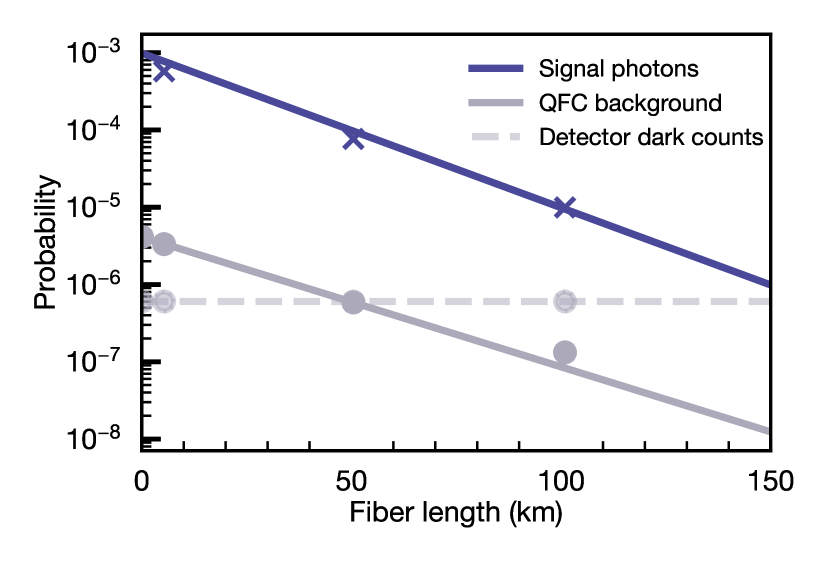
\includegraphics[width=0.84\textwidth]{figures/Zhou2023_Fig8_noise_vs_distance.png}
\caption{链路长度增加时信号与噪声的相对变化示意图。随着距离增加，真实信号计数率指数衰减，而暗计数和部分背景噪声近似保持在固定本底，系统因此会从效率受限逐渐转向噪声受限。该现象提示接口评估不能只做链路损耗预算，而需要把背景与暗计数纳入同一统计框架。图片引自 Zhou 等关于 processing-node 量子网络链路噪声分析的工作。\cite{Zhou2023QuantumNetworkNoise}}
\label{fig:noise_vs_distance}
\end{figure}

\subsection{时间相关效应：滤波记忆、等待与存储退相干}

在实验系统里，很多 ``参数选择'' 实际上都通过时间域起作用。典型例子是滤波：窄带滤波可以抑制 QFC 背景并改善谱重叠，但滤波器（尤其是腔滤波器）本身具有有限响应时间，会在时间域引入尾迹与相关性。\cite{Ikuta2018PolarizationInsensitiveQFC,Pichler2016TimeDelaysMPS} 又例如探测门宽与符合窗：它们看似是电子学设置，但会直接改变 ``被纳入宣告的统计样本''，从而同时影响成功率与条件保真度。\cite{vanleent2022entangling,Zhou2023QuantumNetworkNoise}

这类效应共同指向一个方法学需求：需要能够在同一框架下处理 ``连续时间传播''、``条件化测量'' 与 ``多源噪声'' 的端到端模型。\cite{Reiserer2022CavityEnhancedNetworkNodes,Zhou2023QuantumNetworkNoise} 仅靠把器件效率相乘、再附加一个经验 ``可见度'' 或 ``等效背景率''，通常只能估计量级，却难以回答更接近实验决策的问题：某个滤波带宽为什么会同时改变速率和保真度？长度增加后究竟是等待时间还是假宣告先成为主导瓶颈？这些问题需要显式保留时间相关与条件化测量过程。\cite{Pichler2016TimeDelaysMPS}

\section{本文工作：端到端第一性原理仿真框架与论文结构}[This thesis: end-to-end modeling and organization]

\subsection{为何采用 time-bin 张量网络建模}

从理论上看，本文问题属于连续时间开放量子系统在传播、测量条件化与多尺度噪声下的联合演化。\cite{GardinerCollett1985,Pichler2016TimeDelaysMPS} 将连续时间光场离散为时间 bin 后，系统与光场的逐步相互作用可以写成一维链上的局域更新，从而可以借助矩阵乘积态（matrix product state, MPS）及其时间演化算法 TEBD（time-evolving block decimation）在可管理复杂度下保留关键相干与时间相关信息。\cite{Pichler2016TimeDelaysMPS,Wang2017MPSCascadedQuantumSystems,ArranzRegidor2021WaveguideQED,Yanagimoto2021MPSQuantumPulsePropagation,Yanagimoto2021UltrafastQuantumNonlinearOptics}

对本文的链路而言，这一表示有两点直接好处。第一，接受窗、时间抖动、滤波记忆与点击宣告本来就在时间域定义，time-bin 表示与实验电子学和中继探测逻辑天然对齐。\cite{Pichler2016TimeDelaysMPS,Wang2017MPSCascadedQuantumSystems} 第二，端到端链路包含多个串接环节（发射、QFC、传播、干涉、探测），若在同一时序框架下处理，可把误差源统一映射到 ``最终 POVM/后验态'' 的统计上，从而支持更可解释的误差分解与工作点选择。\cite{vanleent2022entangling,Zhou2023QuantumNetworkNoise}

\subsection{研究内容、边界与章节安排}

基于上述背景，本文聚焦于一条具有明确体系结构指向的中性原子接口链路：两端 $^{87}$Rb 原子在高精细度光学腔中产生原子--光子纠缠，发射的 $780\,\mathrm{nm}$ 单光子经 QFC 转换后进入电信波段，在约 $16\,\mathrm{km}$ 量级的双臂光纤上传输，并在中间站通过两光子干涉与部分 BSM 实现纠缠交换，最终得到两个远程原子之间的 Bell 对。\cite{vanleent2020longdistance,vanleent2022entangling,Ikuta2018PolarizationInsensitiveQFC} 本文关心的重点在于：当多种现实非理想因素同时存在时，这条端到端链路的宣告统计、远程纠缠建立率以及条件态质量如何随参数变化；并进一步分析在不同距离与工作点下，哪些误差源会成为主导瓶颈，从而为实验调参提供可量化依据。

在研究边界上，本文回答的是 ``处理中性原子节点的通信接口能为模块化/分布式量子计算提供怎样的远程纠缠资源''。\cite{Covey2023QuantumNetworksNeutralAtomNodes,Sinclair2024FaultTolerantOpticalInterconnectsNeutralAtoms} 因此，本文聚焦接口链路本身的端到端建模与误差预算，而不试图在绪论阶段把所有更大规模网络协议一次性展开。

全文结构如下：第二章介绍开放量子系统描述、time-bin 离散化、MPS 表示与 TEBD 推进，以及量子信道/测量算符的基本处理框架；第三章建立端到端模型并给出源端发射、频率转换、滤波记忆、光纤传播、模式退化、中继站干涉与探测等环节的建模方法；第四章给出与实验可比对的数值结果与误差预算，重点分析远程纠缠建立率、条件态保真度、Bell 态投影统计及关键参数扫描；结论部分对全文工作进行总结并讨论可能的扩展方向。
